%******************************************************************************************************
%****************************** Second Chapter ********************************************************
%******************************************************************************************************

\chapter{Literature Review}
\label{litrev}

% **************************** Define Graphics Path **************************
\graphicspath{{Chapter2/Figs/}}
% **************************** Define Graphics Path **************************

Now that we have clearly defined objectives, it is necessary to discuss and analyse existing literature that may help to understand and complete our aims.  
%TODO introduce sectino properly


%******************************************************************************************************
%******************************************************************************************************
\section{Dubins Paths}
\label{litrev:dubins}
In 1957, an American mathematician by the name of Lester Dubins 


\begin{figure}[htbp!] 
\centering    
\includegraphics[width=0.5\textwidth]{LSL}
\caption[Dubins LSL Path]{}
\label{fig:lsl}
\end{figure}

\begin{figure}[htbp!] 
\centering    
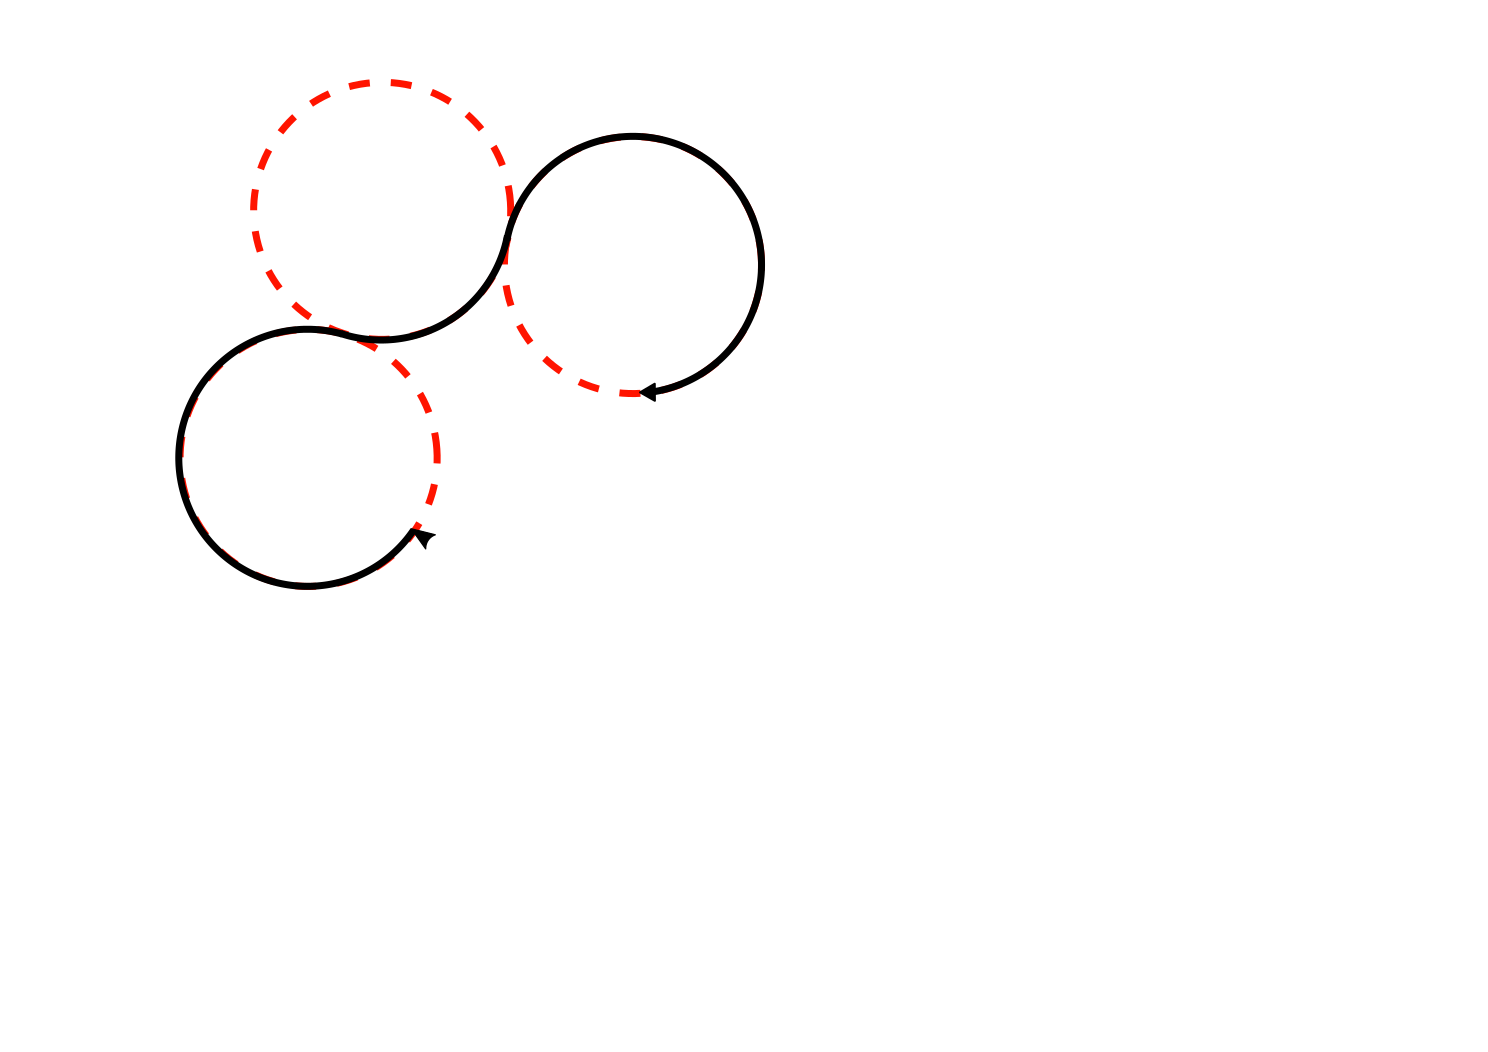
\includegraphics[width=0.5\textwidth]{RLR}
\caption[Dubins RLR Path]{}
\label{fig:rlr}
\end{figure}

\begin{figure}[htbp!] 
\centering    
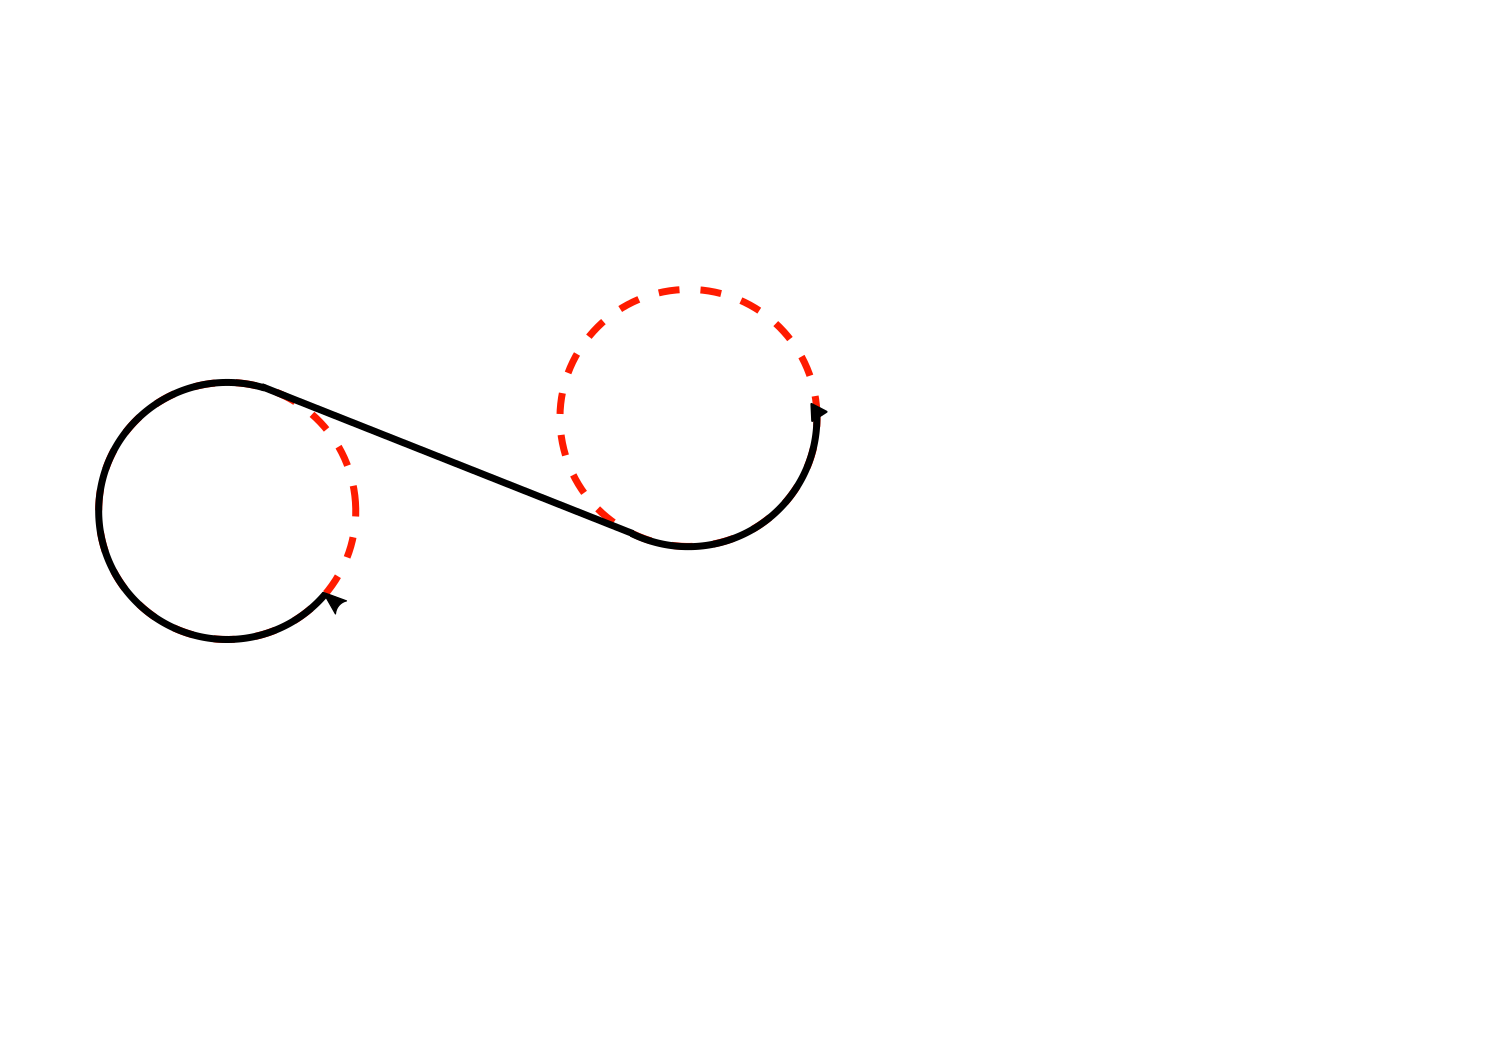
\includegraphics[width=0.5\textwidth]{RSL}
\caption[Dubins RSL Path]{}
\label{fig:rsl}
\end{figure}

%******************************************************************************************************
%******************************************************************************************************
\section{Path Following in Wind}
\label{litrev:path}
